\chapter{Introduction}
\label{chapter:Introduction}


\section{Introductory Example}
\label{section:IntroductoryExample}

\begin{figure}[h!]
\begin{center}
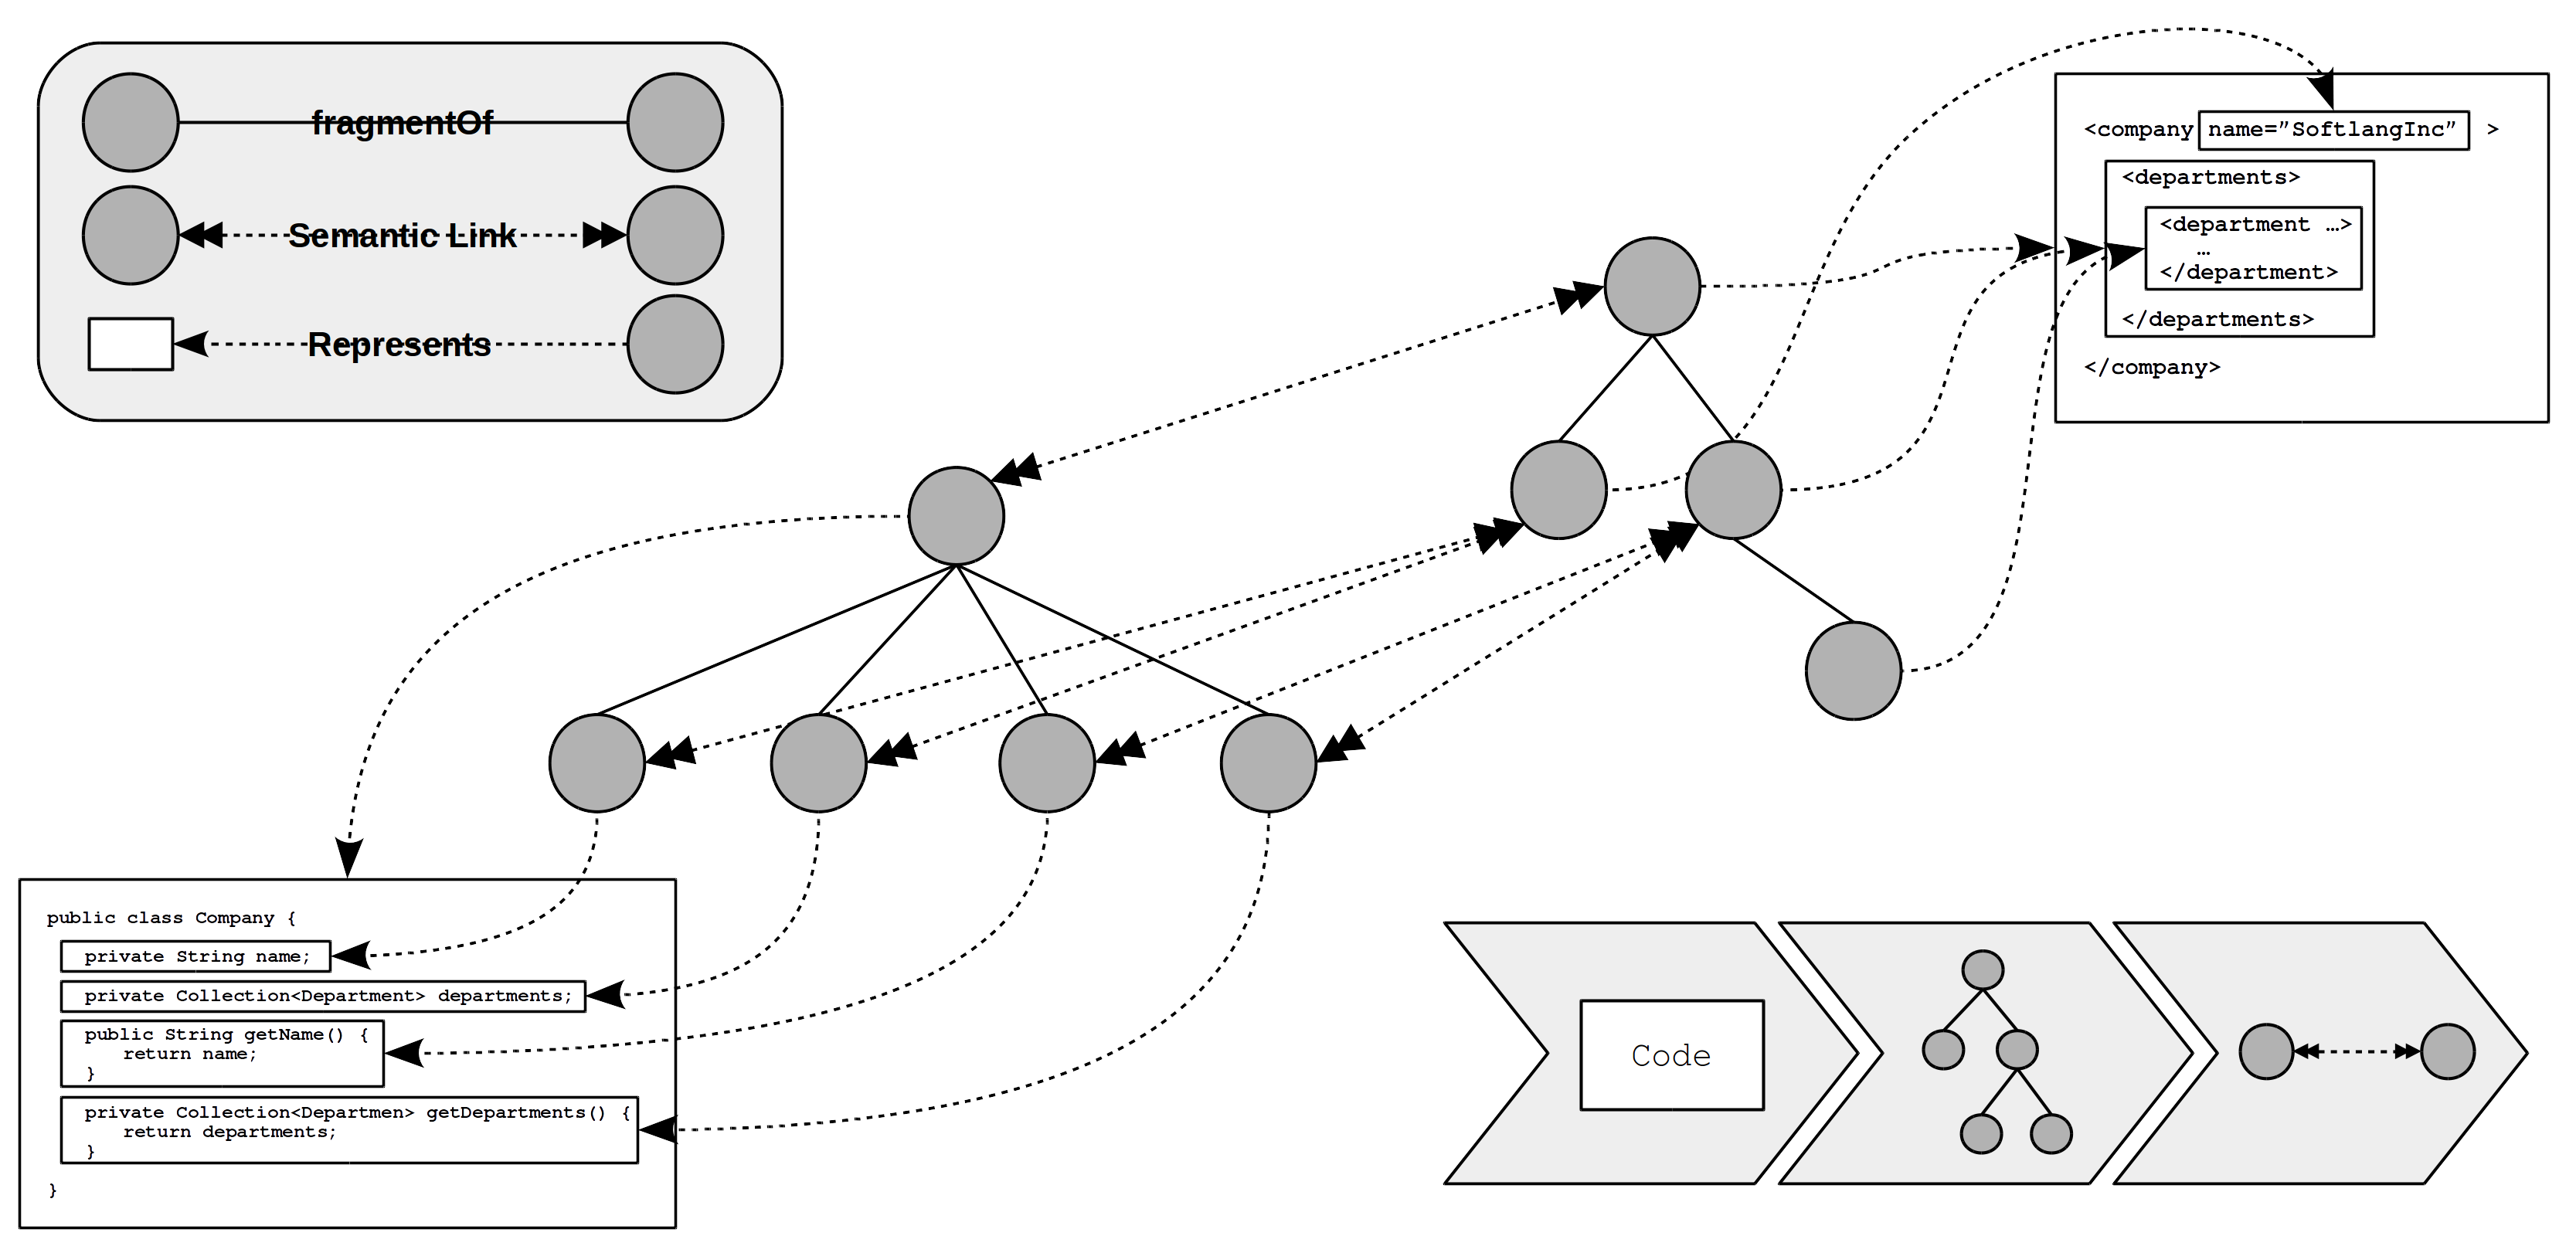
\includegraphics[width=\textwidth]{images/RecoveryExample.png}
\end{center}
\caption{The Example Driven Development Process}
\label{figure:RecoveryExample}
\end{figure}

\section{Contributions \& Non-Contributions}
\label{section:ContributionsAndNonContributions}

\begin{contributions}

\item
This thesis contributes 

\item

\end{contributions}

\begin{noncontributions}

\item
This thesis does not contribute (fundamentally) to the axiomatization of linguistic architectures as described in \cite{DBLP:conf/ecmdafa/LammelV14}, \cite{DBLP:journals/entcs/FavreN05}, \cite{DBLP:conf/sle/Lammel16}, \cite{HeinzLV17}.

\item

\end{noncontributions}

